\documentclass[a4paper]{article}

\usepackage[margin=2cm]{geometry}
\usepackage{fontspec}
\usepackage[catalan]{babel}

\usepackage[hidelinks]{hyperref}
\usepackage{amsmath}
\usepackage{amsfonts}

\usepackage{multirow}

% For figure
\usepackage{float}
\usepackage{tikz}
\usepackage{tikz-dimline}
\usepackage{subfigure}

\setlength{\parindent}{0pt}
\setlength{\parskip}{0.7em}
\def\arraystretch{1.5}

\title{\textsc{Pràctica 2} \\
	\normalsize Aplicació del mètode dels elements finits a l'anàlisi d'una peça prismàtica}

\author{Joan Marcè \and Iñigo Moreno \and Esteve Tarragó}
\date{}

\begin{document}
\maketitle

\section{Introducció}
\subsection{Objectiu}

L'objectiu de la pràctica és realitzar un anàlisi mitjançant el mètode dels elements finits d'una reixa d'embornal metà\l.lica insta\l.lada als accessos d'una nau industrial on hi ha trànsit de vehicles pesats.

\subsection{Dades del problema}
\subsubsection{Condicions del muntatge}
El conjunt a analitzar té 2 parts principals: marc inferior i reixa abatible. El marc inferior està aferrat a l'obra civil i, per tant, és una peça fixa.

La reixa abatible és una peça articulada al marc inferior mitjançant 2 perns. En condicions de servei, la reixa abatible està tancada i recolza sobre el marc inferior. Cal destacar que existeix un petit joc entre les 2 parts del conjunt per tal de permetre i facilitar el tancament de la reixa.

\subsubsection{Geometria}
La reixa abatible a analitzar està formada per un marc, 3 barres longitudinals i 2 orelles d'articulació. A la \autoref{fig:planol} es presenta un dibuix amb les dimensions bàsiques de la reixa.

\begin{figure}[H]
	\centering
	
	\begin{tikzpicture}[scale=0.15]
		% Draw the rectangle
		\filldraw[rounded corners, gray, draw=black] (0,0) -- (65, 0) -- (65, 35) -- (62.5, 35) -- (62.5, 30) -- 
			(2.5, 30) -- (2.5, 35) -- (0, 35) -- cycle;
		\foreach \i in {1,...,4} 
			\draw[fill=white, rounded corners] (2.5,{1.5*\i + (\i - 1)*5.625}) rectangle (62.5, {\i*(5.625+1.5)});
			
		% Draw cotes
		\dimline[extension start length=-4.5cm,
			extension end   length=-4.5cm,
			extension start style={black,thin},
			extension end   style={black,thin}
		]{(2.5, -3)}{(62.5,-3)}{$600$};
		\dimline[extension start length=-6cm,
			extension end   length=-6cm,
			extension start style={black,thin},
			extension end   style={black,thin}
		]{(0,-6)}{(65,-6)}{$630$};
		\dimline[extension start length=4.5cm,
			extension end   length=4.5cm,
			extension start style={black, thin},
			extension end   style={black, thin}
		]{(-4.5,0)}{(-4.5,30)}{$300$};
		\dimline[extension start length=-6cm,
			extension end length=-6cm,
			extension start style={black, thin},
			extension end   style={black, thin},
			line style={arrows=dimline reverse-dimline reverse},
			label style={below=0.8ex}
		]{(68.5, 7.125)}{(68.5,8.625)}{$15$};
		
	\end{tikzpicture}
	\caption{Plànol de la reixa (\emph{mm})}
	\label{fig:planol}
\end{figure}

Com que l'objectiu és analitzar una peça prismàtica, es modelitzarà una barra longitudinal amb les següents dimensions principals (L = 600, b = 15 i h = 40 mm)

\subsection{Material}

La reixa d'embornal està fabricada amb fosa nodular o de grafit esteroïdal (material dúctil). Les característiques del material són les següents:

\begin{table}[H]
	\centering
	\begin{tabular}{|l|c|r|}
		\hline
		\textbf{Característica} & \textbf{Símbol} & \textbf{Fosa nodular FG 38-17} \\
		\hline
		Tensió de ruptura & $f_u$ & 380 MPa \\
		Tensió del límit elàstic & $f_y$ & 235 MPa \\
		Mòdul elàstic o de Young & $E$ & 172000 MPa \\
		Coeficient de Poisson & $\nu$ & 0,275 \\
		\hline
	\end{tabular}
\end{table}

\subsection{Càrrega}
La càrrega màxima que suporta la reixa (P) correspon a la situació en que un grup de rodes d'un vehicle pesat està totalment recolzat sobre la reixa. En aquesta situació, la reixa suporta una massa de 5t.

Com a hipòtesi, es considera que tots els punts de la reixa estan sotmesos a una mateixa càrrega repartida (q), calculada respecte l'àrea neta de la reixa (àrea total menys àrea dels forats) de valor $A_{neta} = 630 \ cm^2$. Es negligeix el pes propi de la reixa.

\section{Qüestions prèvies}
\subsection{Definiu les condicions de contorn de la barra a modelitzar a la part 1}

Com a condicions de contorn es té que la barra està unida pels dos extrems tot i que un d'ells pot lliscar. En aquest cas el costat que romandrà fix serà l'esquerra pel que els desplaçaments del costat esquerra ser

\subsection{Calculeu la càrrega repartida (q)}

La pressió que s'exerceix sobre la reixa serà el pes d'una roda del vehicle (5t) entre l'àrea neta, pel que:
$$
P = \frac{m \cdot g}{A_{neta}} = \frac{5\cdot10^3 \cdot 9,81}{630 \cdot 100} = 0,779\ \frac{N}{mm^2}
$$

Així doncs la càrrega $q$ serà la pressió exercida per l'amplada de la barra pel que:
$$
q = \frac{P}{b} = 0,779 \cdot 15 = \boldsymbol{11,67 \ \frac{N}{mm}} 
$$

\section{Part I: Simulació amb l'element finit plane 182}

\subsection{Anàlisi d'un model amb una malla poc refinada amb 4 elements i 10 elements en longitud (4x10 = 40 elements finits)}

\textbf{Anàlisi de la deformada i del desplaçament vertical màxim ($\delta_{y, \max}$)}

\begin{figure}[H]
	\subfigure[Deformació]{
		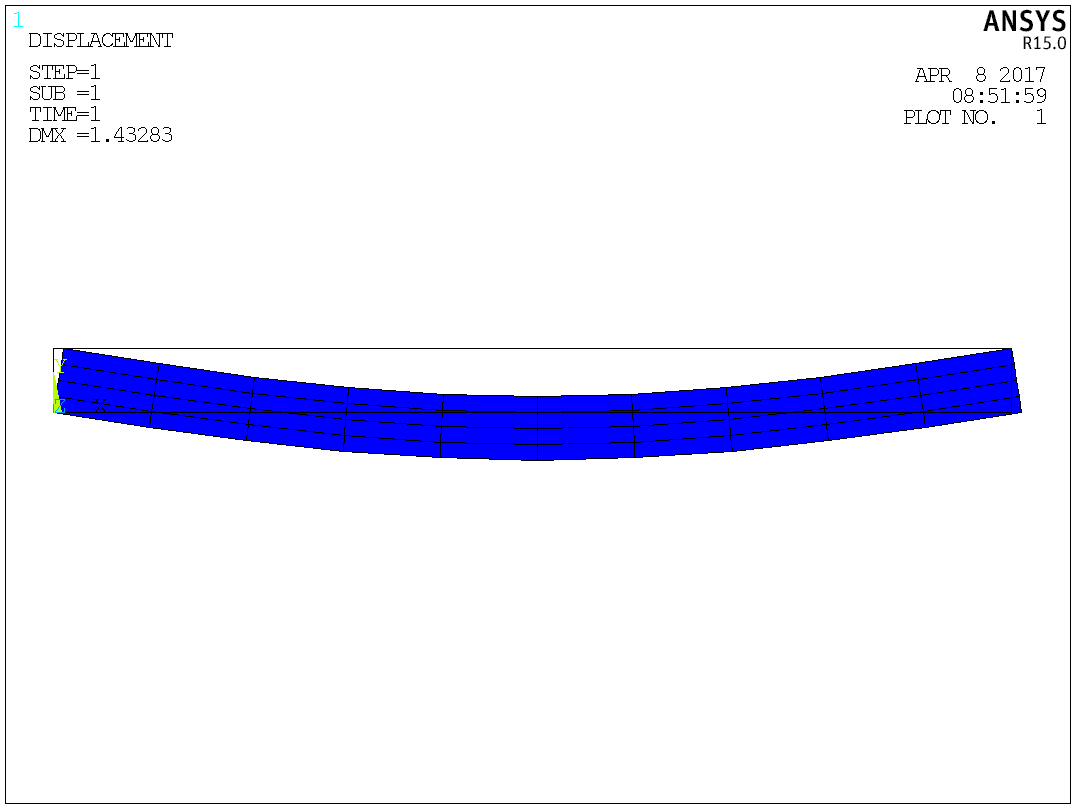
\includegraphics[width=0.49\textwidth]{images/40_deformed}
	}
	\label{fig:40_deformed}
	\hfill
	\subfigure[Mapa de desplaçaments verticals UY]{
		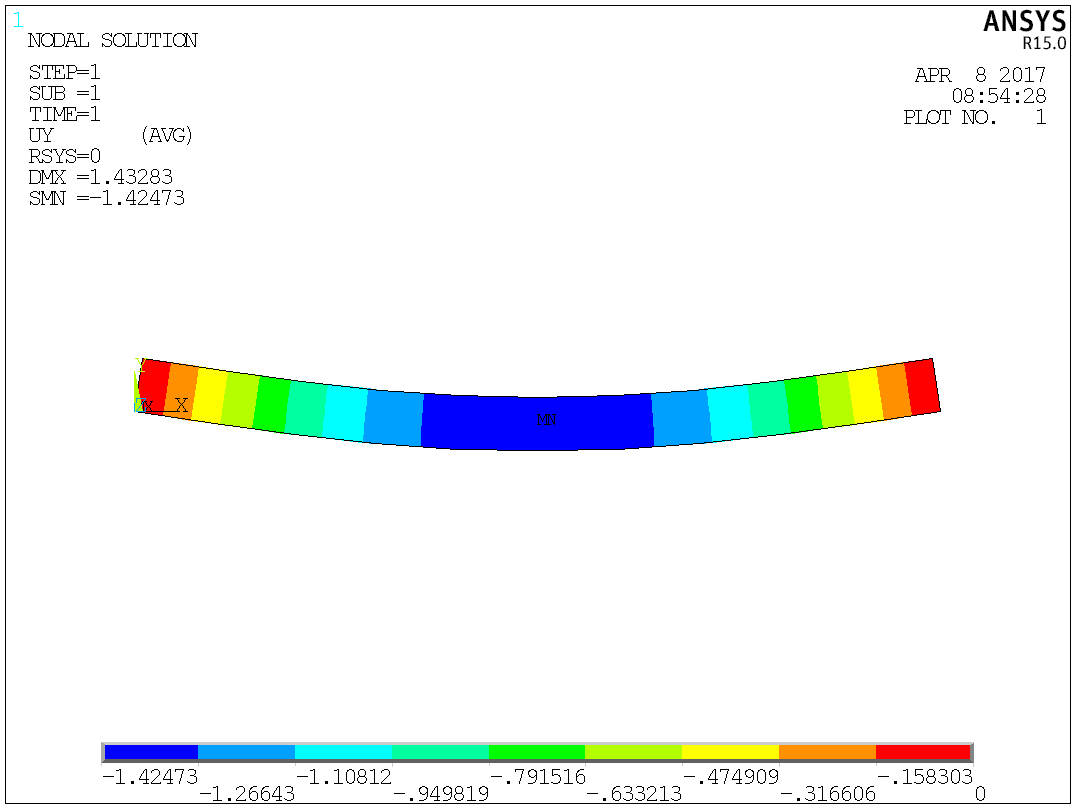
\includegraphics[width=0.49\textwidth]{images/40_UY}
	}
	\label{fig:40_UY}
	\caption{Resultats del desplaçament}
	\label{fig:40_displacement}
\end{figure}

\textbf{Anàlisi de les tensions normals ($\sigma_x$)}

\textbf{Anàlisi de les tensions tangencials ($\tau_{xy}$)}

\textbf{Càlcul del coeficient de seguretat de la peça (criteri de Von Mises)}

\subsection{Anàlisi d'un model amb una malla refinada amb 10 elements en alçada i 40 elements en longitud (10x40 = 400 elements finits)}
\textbf{Anàlisi de la deformada i del desplaçament vertical màxim ($\delta_{y,\max}$)}

\textbf{Anàlisi de les tensions normals ($\sigma_x$)}

\subsection{Comparació dels resultats obtinguts amb els resultats teòrics}

\begin{table}[H]
	\centering
	\begin{tabular}{|l|c|r|r|r|}
		\cline{4-5}
		\multicolumn{3}{c|}{\multirow{2}{*}{}} & \textbf{Malla poc refinada} & \textbf{Malla refinada} \\
		\multicolumn{3}{c|}{} & 4x10 = 40 elements & 10x40 = 400 elements \\
		\hline
		\textbf{Paràmetre} & \textbf{Unitats} & \textbf{Solució teòrica} & \textbf{Valor} & \textbf{Valor} \\
		\hline
		$\sigma_{x,\max+}$ & $N/mm^2$ & 133,31 & 128,86 & 131,37 \\
		$\sigma_{x,\max-}$ & $N/mm^2$ & -133,31 & -128,86 & -131,37 \\
		$\tau_{xy,\max+}$ & $N/mm^2$ & 8,88 & 7,2 & 9,24 \\
		$\tau_{xy,\max-}$ & $N/mm^2$ & -8,88 & -7,2 & -9,24 \\
		$\delta_{y,\max}$ & $mm$ & 1,45 & 1,42 & 1,45 \\
		\hline
	\end{tabular}
\end{table}



\subsection{Anàlisi d'un model amb una malla refinada amb 10 elements }

\section{Part 2: Simulació amb l'element finit BEAM 188}
\textbf{Anàlisi de la deformada i del desplaçament vertical màxim ($\delta_{y,max}$)}

\textbf{Anàlisi del diagrama de moments flectors ($M_z$)}

\textbf{Anàlisi del diagrama d'esforços tallants ($T_y$)}


\end{document}